\section{Photodetectors}\label{sec:photodetectors}
\subsection{Photo-multipliers}
Photomultipliers (PMTs) are based on the external photoelectric effect and on secondary electron emission. A standard PMT is an evacuated glass tube containing a \textbf{photocathode}, a series of \textbf{dynodes}, and an \textbf{anode}.

Electrons emitted by the photocathode are accelerated by a potential difference $\Delta V$ toward the first dynode, where they generate secondary electrons by impact. The typical secondary emission factor is $\delta \approx 3-10$. These electrons are then accelerated to the next dynode, where the process is repeated. After $n$ dynodes, the number of electrons reaching the anode is approximately
\[
G = \delta^n \approx 10^5-10^7 \equiv \text{current amplification or gain}.
\]

In practice, the total gain also depends on the collection efficiency of the electron cascade, but the estimate above captures the main amplification mechanism. The current collected by the anode flows through a load resistor and produces an output voltage signal.
A sufficiently high bias voltage must be applied in order to extract electrons efficiently from the photocathode and accelerate them toward the dynodes.

\subsubsection{PMTs' general properties}
For a photomultiplier we have:
\begin{itemize}
    \item \textbf{Spectral range:} this \hl{indicates the range of wavelengths to which the device is sensitive}. In practice, it depends both on the \textit{photocathode material}, which determines the photoemission threshold, and on the \textit{input window}, which must transmit the incoming light efficiently. A PMT is typically sensitive from the ultraviolet to the visible and, for special photocathodes, up to the near infrared. This quantity is important because it tells us which optical signals can be detected by the device.
    If we study the \textbf{photocathode responsivity}, we observe that for large wavelengths $\lambda$, the photon energy $E = h\nu = hc/\lambda$ becomes too small to eject electrons from the photocathode, so the absorption efficiency drops. As $\lambda$ decreases, the photon energy increases and the responsivity grows, but at sufficiently short wavelengths a cutoff appears. This cutoff is mainly due to the transmission properties of the input window and, in some cases, to the absorption properties of the photocathode material itself. In other words, the spectral response is determined both by the photon energy threshold for photoemission and by the optical transmission of the detector window.
\begin{figure}[H]
    \centering
    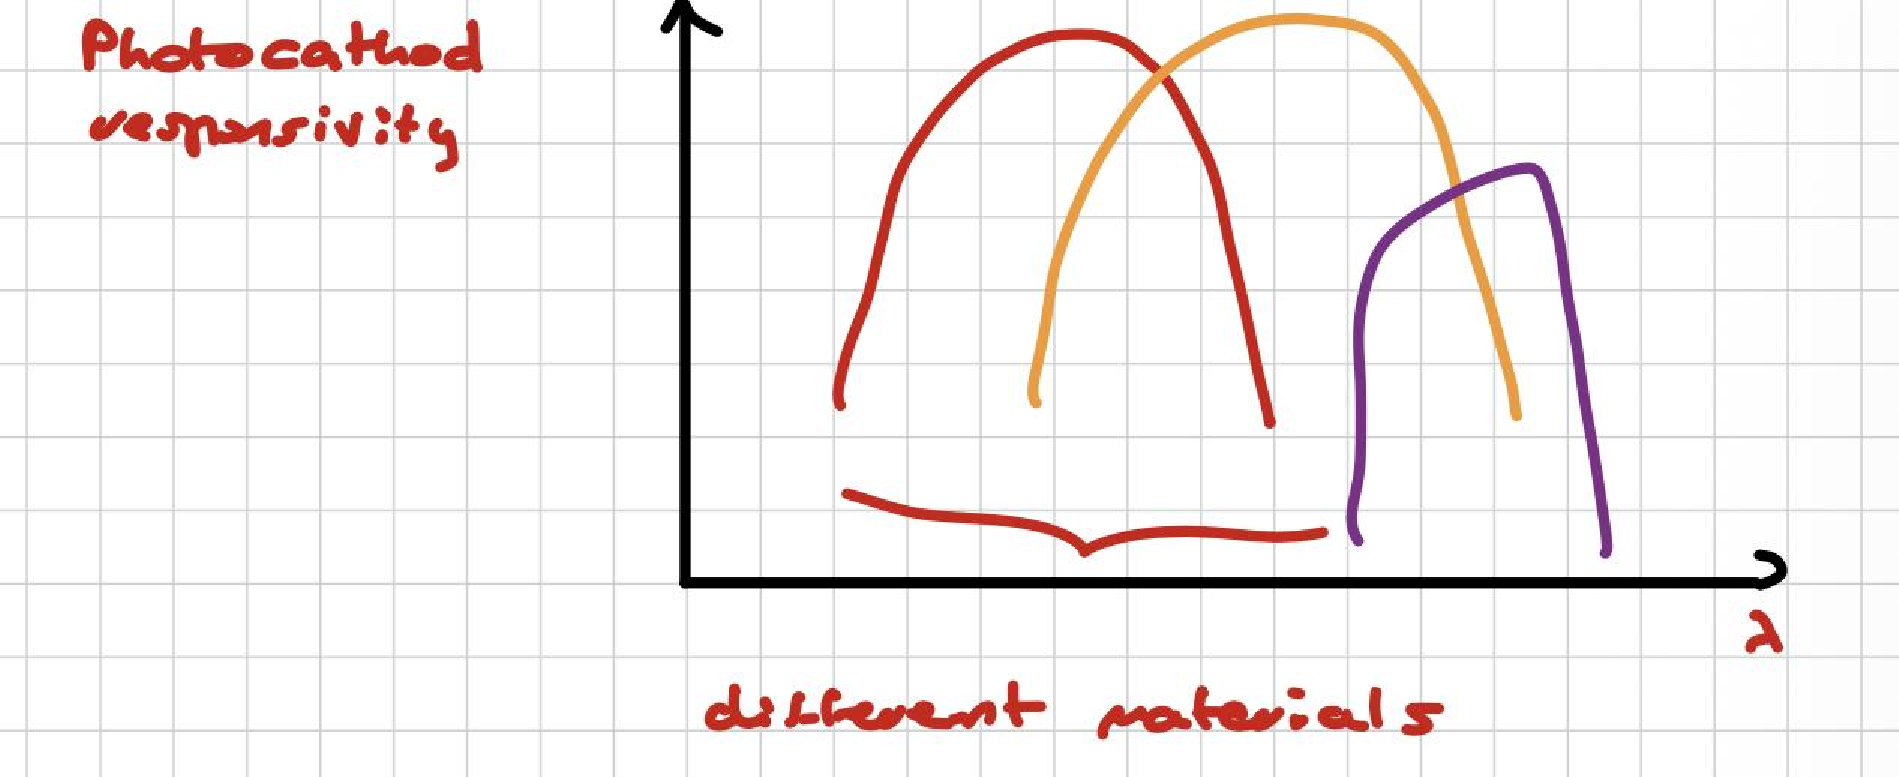
\includegraphics[width=0.8\linewidth]{images_in_pdf/8-/Grafico_39.pdf}
\end{figure}

    \item \textbf{Anode sensitivity:} $K(\lambda)$.
    \begin{equation}\label{eqn:8-photomultiplier-anode-sensitivity}
    \begin{aligned}
    K(\lambda)
    &= \frac{\text{output signal}}{\text{incident radiation power}} =\\[0.5ex]
    &= \frac{S}{\Phi}
    = \frac{S}{I(\mathrm{W/cm^2})\cdot A(\mathrm{cm^2})}
    \hspace{0.4cm}\left[\frac{A}{W}\right]
    \approx 10^3-10^5 \frac{A}{W}.
    \end{aligned}
    \end{equation}

    This quantity measures how efficiently the photomultiplier converts incident optical power into an electrical output signal at a given wavelength. A \hl{larger sensitivity means that a smaller optical power is needed to produce a measurable current}.

    \item \textbf{Quantum efficiency:} $\eta \approx 0.1-50\%$.\\
    The quantum efficiency is the probability that an incoming photon actually produces a photoelectron at the photocathode. It tells us how effective the first step of the detection process is. A higher quantum efficiency means that a larger fraction of the incident photons contribute to the output signal, which is \hl{crucial when measuring weak light}.

    \item \textbf{Maximum anode current:} $\approx 10-100\,\mu A$.\\
    This is the largest current that can be collected at the anode without significantly degrading the performance of the detector. Above this value, heating effects, gain saturation, and possible damage to the device may occur. It sets the upper limit of the dynamic range.

    \item \textbf{Dark current:} $I_d$.\\
    This is the current measured even in complete darkness. It is mainly due to thermionic emission from the photocathode or from the dynodes, and it therefore \hl{increases with temperature}. Since it acts as a false signal, it limits the minimum detectable light level. For this reason, photomultipliers operating in the near infrared are often cooled to reduce dark current.

    \item \textbf{Noise equivalent power:} $\NEP$.\\
    This is the incident optical power that produces an output signal equal to the root-mean-square value of the intrinsic noise of the detector. It is therefore a measure of the weakest detectable optical signal. A smaller $\NEP$ means a more sensitive detector.
    The detected noise increases with the transmission bandwidth $\Delta f$ and scales as $\sqrt{\Delta f}$:
    \begin{equation}\label{eqn:8-photomultiplier-NEP}
    N = K(\lambda)\cdot \NEP \cdot \sqrt{\Delta f}
    \hspace{1cm}
    \NEP = \frac{\sqrt{2e\,I_d\,G}}{K(\lambda)}
    \hspace{0.3cm}\left[\frac{\mathrm{W}}{\sqrt{\mathrm{Hz}}}\right].
    \end{equation}
    
    This expression shows that the $\NEP$ increases when the dark current increases, because the intrinsic noise becomes larger. It also depends on the gain $G$ and on the responsivity $K(\lambda)$.
    The ratio $\frac{S}{N}=1$ when the incident optical power is equal to the $\NEP$; signals weaker than the $\NEP$ are buried in the noise. For $\Delta f \approx 1\,\mathrm{Hz}$, one typically finds $\NEP \approx 10^{-16}-10^{-15}$.

    \item \textbf{Detectivity:} $D = \frac{1}{\NEP}$.\\
    Detectivity is simply the inverse of the $\NEP$. It is useful because a larger detectivity corresponds to a more sensitive detector.

    \item \textbf{Normalized detectivity:} $D^\star$.
    \begin{equation}\label{eqn:8-photomultiplier-normalized-detectivity}
    D^* = \frac{\sqrt{A}}{\NEP} = D\cdot \sqrt{A}
    \hspace{0.4cm}
    \left[\frac{\mathrm{cm}\cdot \sqrt{\mathrm{Hz}}}{\mathrm{W}}\right],
    \end{equation}

    where $A$ is the active area of the device. This quantity is used to compare detectors of different sizes, since it normalizes the detectivity with respect to the detector area.
\end{itemize}


\subsubsection{PMTs' noise sources}
\hl{The total noise of the photomultiplier has several components}, classified as follows:
\begin{enumerate}
    \item \textbf{Shot noise of the photocathode:} the number of detected photoelectrons fluctuates around an average value. For a classical source with Poissonian statistics, the current generated by the detector also fluctuates around its mean value, with rms fluctuations scaling as the square root of the average number of detected events.

    \item \textbf{Excess noise due to secondary electron emission:} the dynode multiplication process is not perfectly deterministic, so the gain itself fluctuates from event to event.

    \item \textbf{Johnson noise in the load resistor:} this is the thermal noise associated with the resistance in the readout circuit.
\end{enumerate}

\calloutwarn{%
Practical downsides of photomultipliers:
\begin{itemize}
    \item They are sensitive, fragile, and expensive.
    
    \item They must be stored in a light-tight box.
    
    \item They require a warm-up time of about $90$ minutes for the operating parameters to stabilize.
    
    \item The bias voltage should not be changed unnecessarily, because it modifies the gain and the response of the device.
    
    \item They require magnetic shielding to protect the electron trajectories from external magnetic fields.
\end{itemize}
}

\subsection{Avalanche photodiodes}
Avalanche photodiodes (APDs) are based on the internal photoelectric effect, i.e. the generation of electron--hole pairs by photon absorption in a semiconductor. These carriers are separated and accelerated by an electric field $\vec{E}$ established across a reverse-biased p--n junction (often in a p-i-n configuration). \calloutinfo{%
Compared to photomultipliers, APDs offer a wider spectral range and a compact solid-state design.
}
The photocarrier multiplication is achieved internally through impact ionization, leading to a gain of $G \approx 10-500$ in linear mode.
\begin{figure}[H]
    \centering
    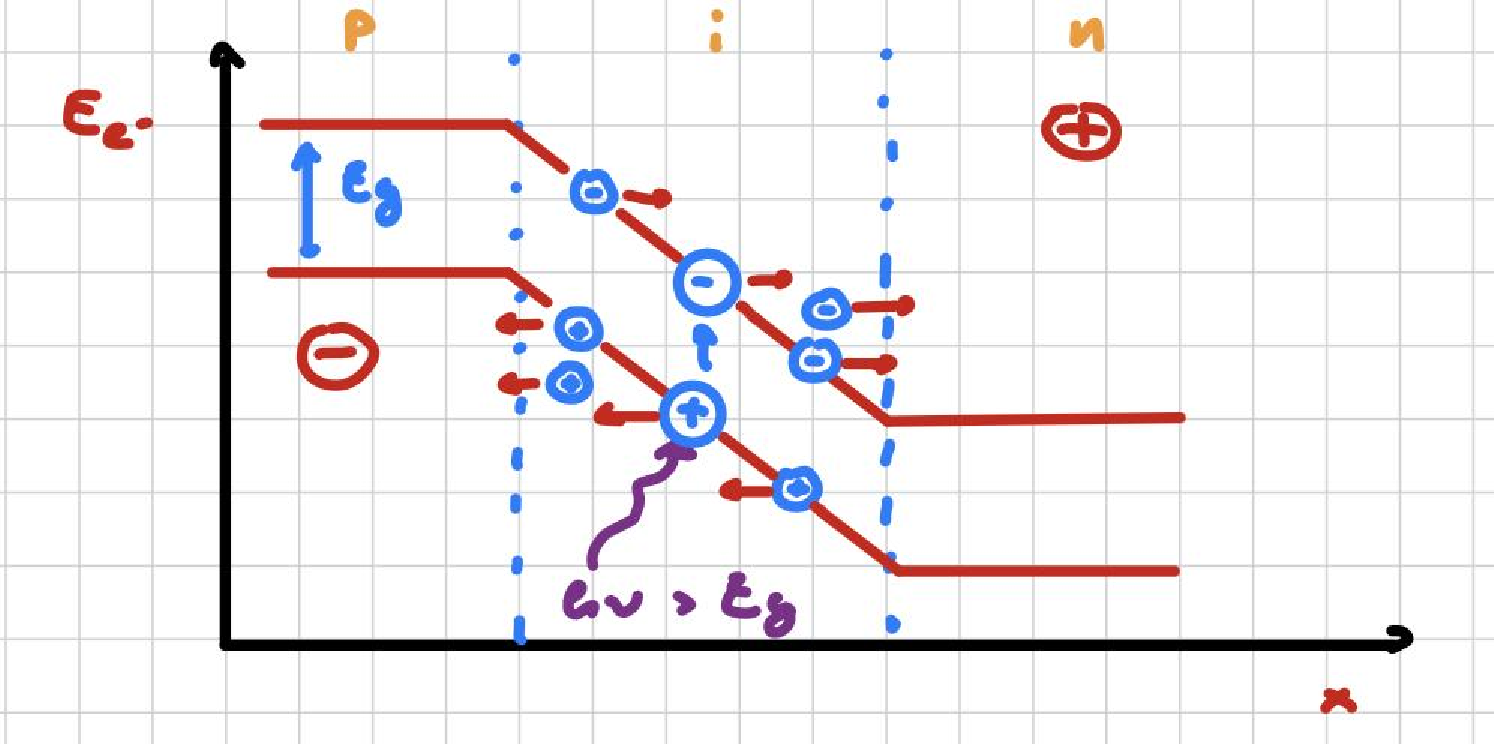
\includegraphics[width=0.8\linewidth]{images_in_pdf/8-/Grafico_40.pdf}
\end{figure}

\subsubsection{APDs' working principle}
\begin{itemize}
    \item A p--n junction is operated under reverse bias, creating a strong electric field in the depletion region.
    \item An incident photon with energy $E = h\nu > E_g$ is absorbed, generating an electron--hole pair.
    \item The electric field $\vec{E}$ accelerates electrons and holes in opposite directions.
    \item If $\vec{E}$ is sufficiently strong, carriers gain enough kinetic energy to ionize atoms by impact, generating additional electron--hole pairs. This leads to an avalanche multiplication process.
\end{itemize}

However, \hl{two main issues arise}:
\begin{enumerate}
    \item \textbf{Carrier multiplication noise and breakdown.}\\
    Both electrons and holes can contribute to impact ionization, which introduces fluctuations in the gain and may lead to uncontrolled avalanche breakdown. To describe this, we define the \textbf{ionization coefficient} $\alpha_i$, i.e. the number of ionization events per unit distance, and the \textbf{ionization ratio}:
    \begin{equation}\label{eqn:8-avalanche-photodiode-ionization-ratio}
    k = \frac{\alpha_h}{\alpha_e}
    \hspace{2ex}
    \begin{cases}
    k \to 0 \Rightarrow \text{electron-dominated multiplication};\\
    k \to \infty \Rightarrow \text{hole-dominated multiplication}.
    \end{cases}
    \end{equation}

    Materials with strongly asymmetric ionization coefficients (small $k$ or large $k$) are preferred, since they reduce the multiplication noise.

    \item \textbf{Trade-off between absorption and electric field.}\\
    A thick intrinsic region improves photon absorption and thus quantum efficiency, while a thin region is required to achieve a strong electric field for avalanche multiplication. This conflict is solved by engineering the device structure, typically separating it into:
    \begin{itemize}
        \item[--] an \textit{absorption layer} (low electric field),
        \item[--] a \textit{multiplication layer} (high electric field).
    \end{itemize}
\end{enumerate}

\subsubsection{APDs' general properties}
\calloutwarn{%
APDs are compact, robust, and less fragile than photomultipliers, but generally exhibit higher noise due to the stochastic nature of the multiplication process.
}
\begin{itemize}
    \item \textbf{Dark noise:}
    \begin{equation}\label{eqn:8-avalanche-photodiode-dark-noise}
    N_{A.P.} = \sqrt{2e\, I_d\, G_{A.P.}^2\, F(G_{A.P.})\, \Delta f}.
    \end{equation}
    Here $G_{A.P.}$ is the avalanche gain, and the factor $G^2$ reflects the amplification of current fluctuations. $F(G)$ is the \textbf{excess noise factor}, which accounts for the statistical nature of impact ionization and depends strongly on the ionization ratio $k$. The dark current $I_d$ includes thermal generation and tunneling contributions.

    \item \textbf{Noise equivalent power:}
    \begin{equation}\label{eqn:8-avalanche-photodiode-NEP}
    \NEP = \frac{\sqrt{2e\, I_d\, G_{A.P.}^2\, F(G_{A.P.})}}{K_{A.P.}(\lambda)}.
    \end{equation}

    This represents the minimum detectable optical power and shows explicitly how the avalanche process increases noise through both $G$ and $F(G)$.

    \item \textbf{Normalized detectivity:}
    \begin{equation}\label{eqn:8-avalanche-photodiode-normalized-detectivity}
    D^* = \frac{\sqrt{A}\, K_{A.P.}(\lambda)}{\sqrt{2e\, I_d\, G_{A.P.}^2\, F(G_{A.P.})}}
    \hspace{0.4cm}
    \left[\frac{\mathrm{cm} \cdot \sqrt{\mathrm{Hz}}}{\mathrm{W}}\right].
    \end{equation}

    For silicon APDs, typical values are $D^* \sim 10^{12}-10^{13}$, significantly lower than photomultipliers, so that:
    \begin{equation}
    \frac{D^*_{P.M.}}{D^*_{A.P.}} \approx 10-100.
    \end{equation}
    
    \item \textbf{Spectral response:} the response typically exhibits a bell-shaped curve.
    \begin{figure}[H]
    \centering
    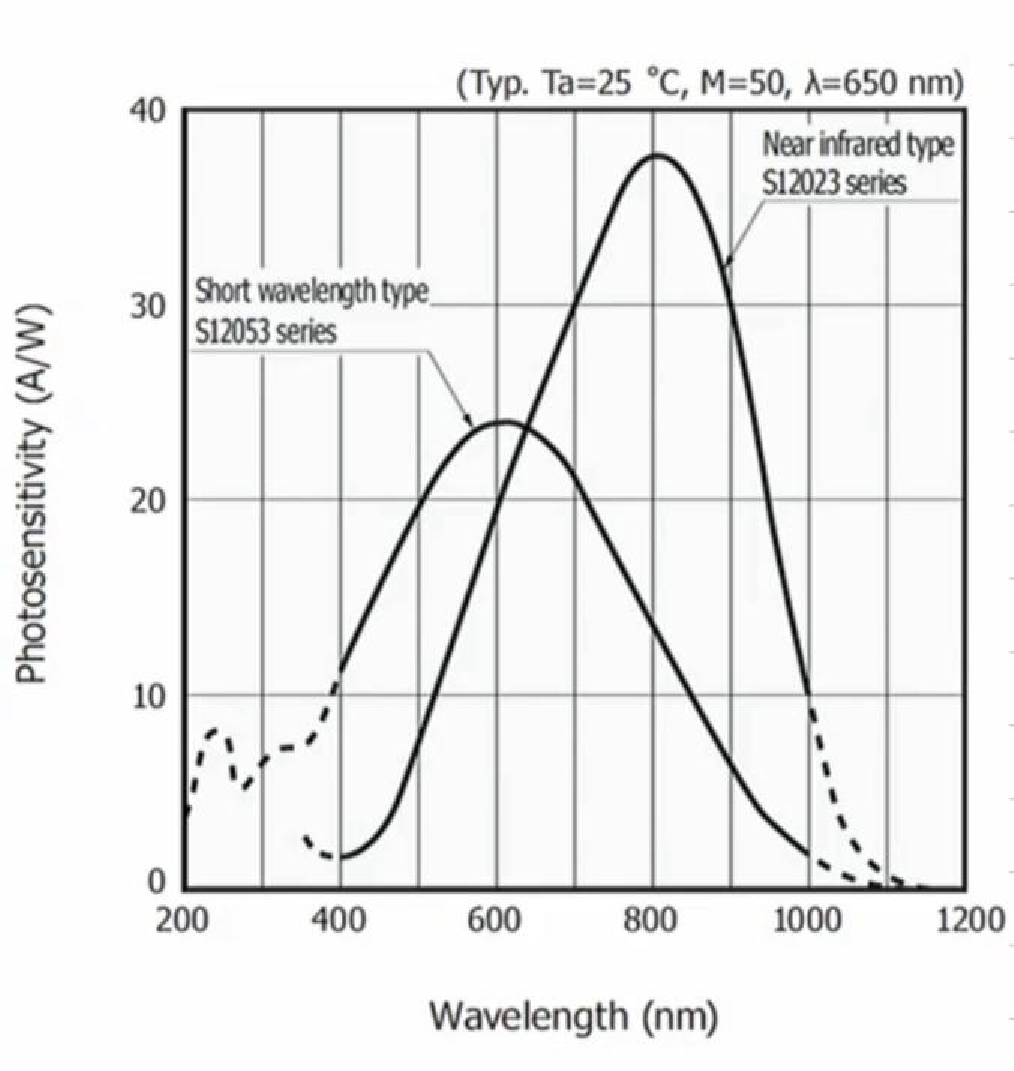
\includegraphics[width=0.4\linewidth]{images_in_pdf/8-/Grafico_41.pdf}
    \end{figure}

    This behavior can be understood as follows:
    \begin{itemize}
        \item For large wavelengths ($\lambda$ high), photon energy is too low ($h\nu < E_g$), so absorption is not possible.
        \item For short wavelengths, the penetration depth is lower and the photons are absorbed very close to the surface, where recombination processes reduce carrier collection efficiency (less multiplication processes).
        \item At intermediate wavelengths, absorption occurs efficiently within the depletion region, maximizing the signal.
    \end{itemize}
\end{itemize}
\subsubsection{APDs' working principle in Geiger mode}
\calloutinfo{%
APDs are also used for very low light detection, including single-photon counting, in the so-called \textbf{Geiger mode}. In this regime, the device is biased above the breakdown voltage, and the gain reaches $G \approx 10^5-10^6$. In this condition, a single absorbed photon can trigger a macroscopic current pulse.
}

\begin{figure}[H]
    \centering
    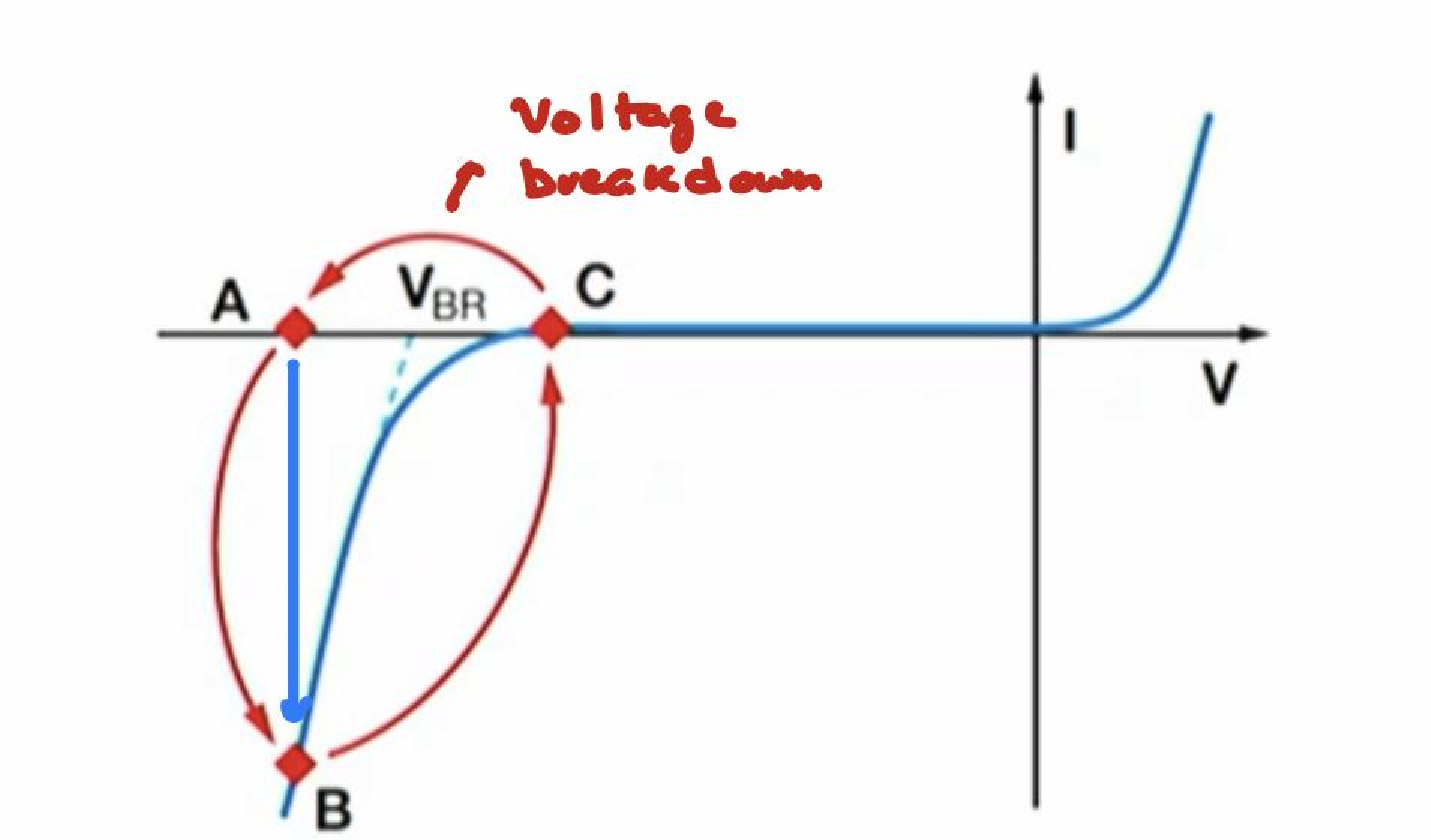
\includegraphics[width=0.6\linewidth]{images_in_pdf/8-/Grafico_42.pdf}
\end{figure}

\begin{enumerate}
    \item The bias voltage is raised to point A, corresponding to a metastable state above breakdown. A single photon absorption can trigger a large avalanche current (point B), producing a detectable pulse.
    
    \item A quenching circuit rapidly lowers the voltage from point B to point C (below the breakdown voltage $V_{BR}$), stopping the avalanche.
    
    \item The voltage is then restored to point A during the so-called \textbf{dead time}, during which the detector is insensitive. In this phase:
    \begin{itemize}
        \item spontaneous avalanches may occur, contributing to the dark count rate;
        
        \item trapped charges in defects may be released later, producing correlated pulses known as \textbf{afterpulses}.
    \end{itemize}
\end{enumerate}
\subsection{Superconducting nanowire single-photon detectors (SNSPDs)}
These detectors are the preferred choice in many landmark experiments and have become a standard tool in quantum communication and quantum computing because of their excellent performance: very high detection efficiency, extremely low dark-count rates, and very short timing jitter. Here, \textbf{time jitter} is the statistical spread of the delay between the arrival of a photon at the detector and the generation of the electrical pulse. A smaller jitter corresponds to a better time resolution.

\subsubsection{SNSPDs' working principle}
\begin{itemize}
    \item The detector must be operated at cryogenic temperature, so that the nanowire remains below the critical temperature $T_C$.
    
    \item When a photon is absorbed by the nanowire, its energy is deposited locally and creates a \textit{hotspot}. This process breaks Cooper pairs and generates quasiparticles.
    
    \item The hotspot locally suppresses superconductivity. If the bias current density becomes larger than the critical current density in that region, i.e. $j > j_c$, a resistive barrier forms.
    
    \item The bias current is then diverted into the external readout circuit, producing a voltage pulse. After a short time, the hotspot cools down and the nanowire returns to the superconducting state.
\end{itemize}
The resistance spike is typically on the order of $\mathrm{k}\Omega$ and is much larger than the input impedance of the readout amplifier, which is typically about $50\,\Omega$. As a consequence, most of the bias current $I_b$ is diverted to the readout circuit, and a measurable voltage pulse is generated.

\begin{figure}[H]
    \centering
    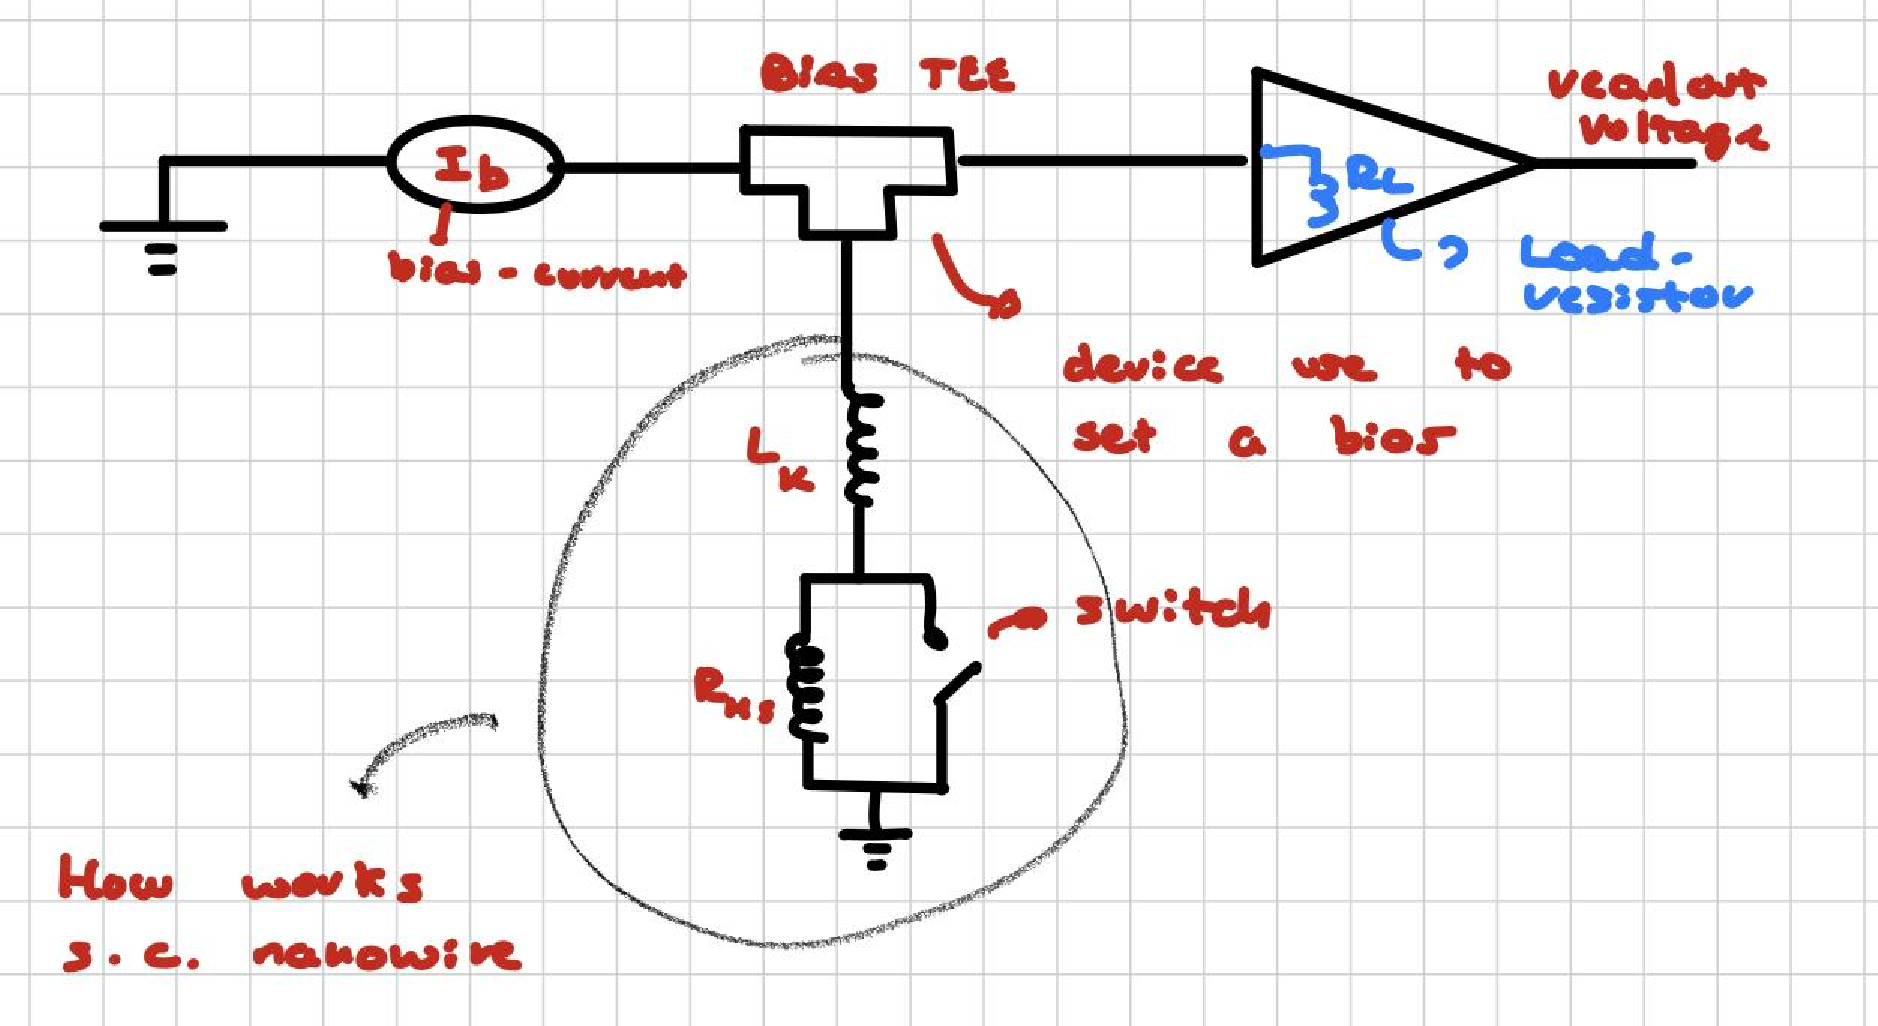
\includegraphics[width=0.8\linewidth]{images_in_pdf/8-/Grafico_43.pdf}
\end{figure}

In the superconducting regime the hotspot resistance satisfies $R_{HS} \approx 0$, while after photon absorption the local resistance becomes finite, $R_{HS} \approx \unit{\kilo\ohm}$, and the current is shunted to the amplifier, producing the output pulse.
\begin{figure}[H]
    \centering
    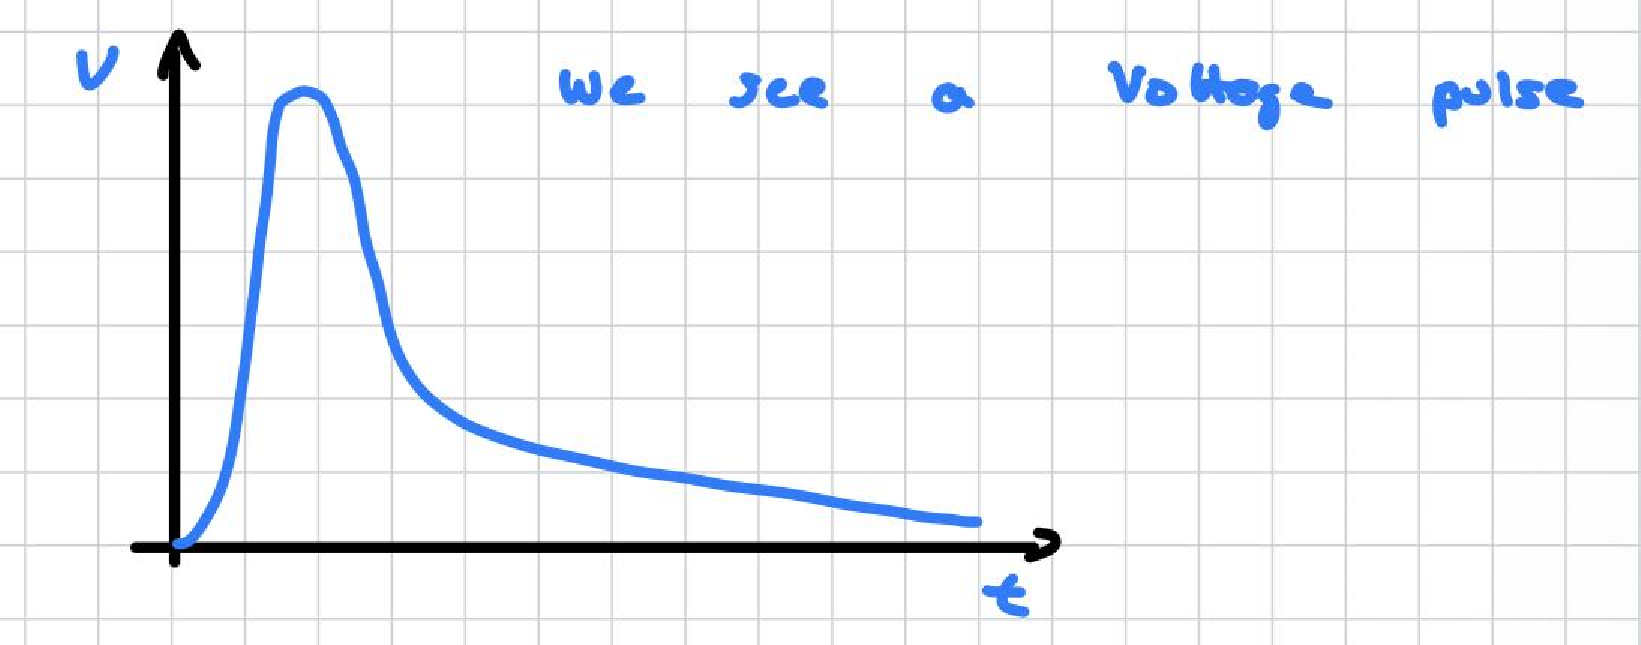
\includegraphics[width=0.8\linewidth]{images_in_pdf/8-/Grafico_44.pdf}
\end{figure}

The current flowing toward the readout circuit is governed by the circuit inductance, and the pulse decay is typically described by a time constant of the form
\[
\tau \sim \frac{L_k}{R_{HS}} \approx \mathrm{ms},
\]
where $L_k$ is the kinetic inductance of the nanowire and $R_{HS}$ is the hot-spot resistance. The recovery of the superconducting state depends on how quickly the hotspot cools down, typically the time constant goes as:
\[\tau \sim \frac{L_k}{R_L}\]
with $R_L \approx \qty{50}{\ohm}$ 

\calloutwarn{%
If the resistive region does not cool sufficiently fast, the detector can enter a \textbf{latching} regime, in which it remains trapped in a resistive state and cannot detect new photons.
}

\subsubsection{SNSPDs' fabrication and spectral response}

Different superconducting materials can be used, each with its own critical temperature and energy gap. The fabrication typically proceeds as follows:
\begin{itemize}
    \item A dielectric layer is deposited on a silicon wafer together with an optical cavity, usually designed as a quarter-wave structure, and a thin superconducting film. The optical cavity maximizes the absorption probability in the superconducting layer.
    \item Electron-beam lithography is then used to pattern the superconducting film into a nanowire and to define the electrical contacts.
    \item After the electrical contacts are fabricated, optical coupling is realized by aligning an optical fiber precisely above the nanowire, which requires a very high coupling efficiency.
    \item The final device is compact, robust, and highly sensitive, but it must be operated with dedicated cryogenic equipment.
\end{itemize}
The superconducting energy gap sets a limit on the detectable wavelength. In practice, one can identify different wavelength windows, and the optical cavity can be engineered to maximize absorption in the desired spectral region.
\begin{figure}[H]
    \centering
    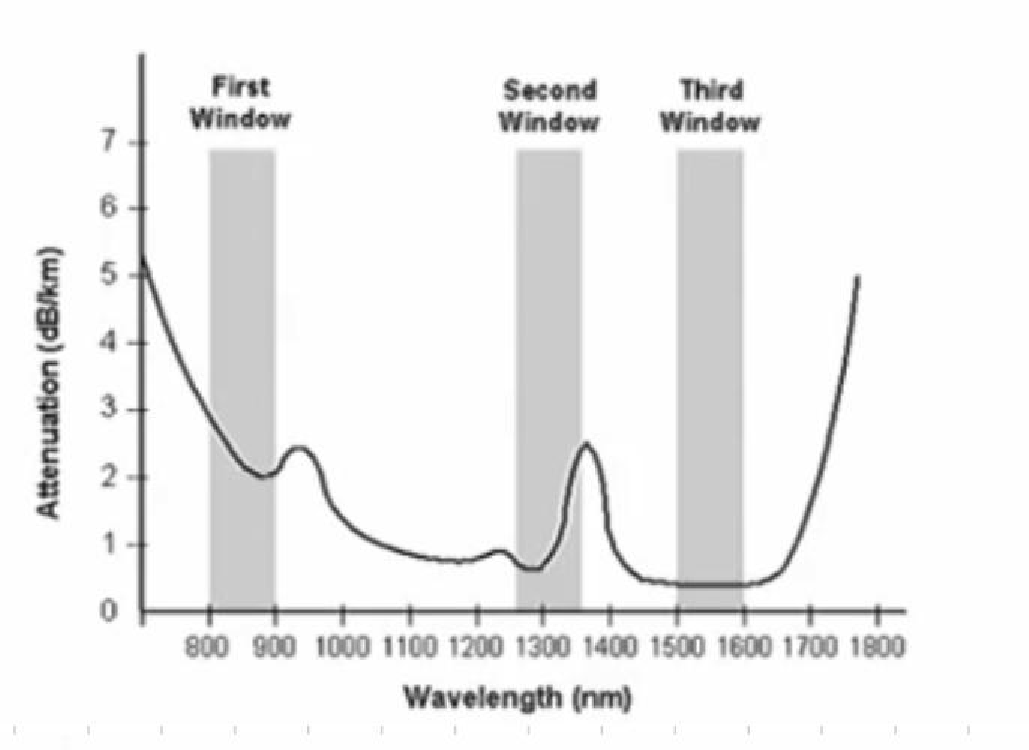
\includegraphics[width=0.8\linewidth]{images_in_pdf/8-/Grafico_45.pdf}
\end{figure}

\begin{figure}[H]
    \centering
    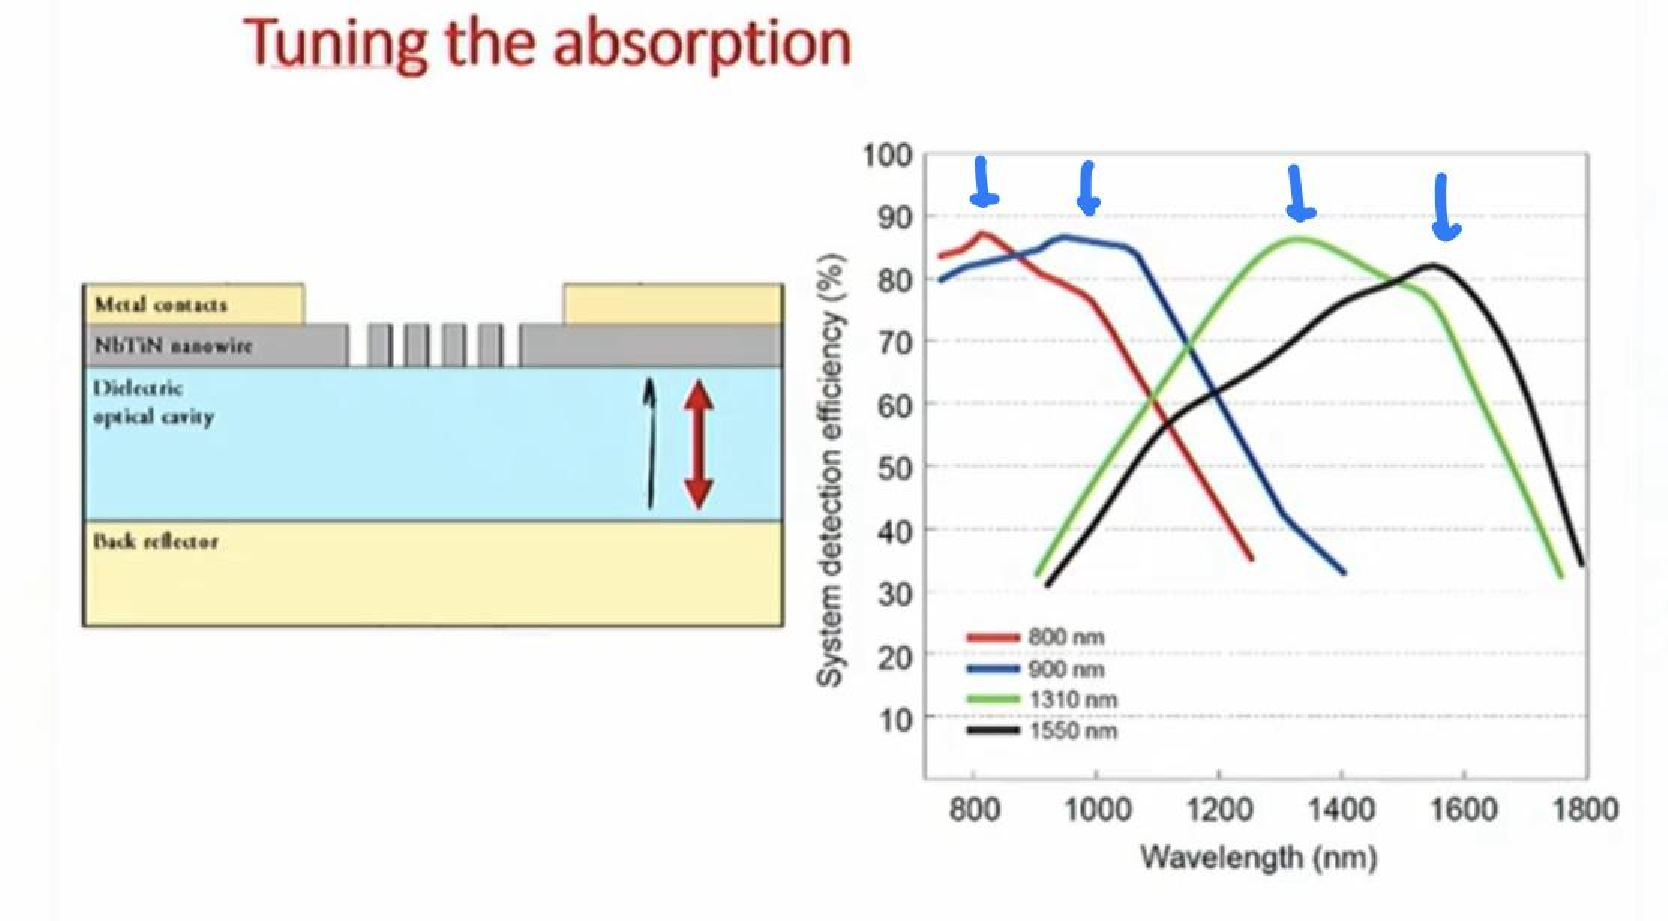
\includegraphics[width=0.8\linewidth]{images_in_pdf/8-/Grafico_46.pdf}
\end{figure}

When $\lambda$ is in the infrared range, the dark-count rate increases because blackbody radiation from the room and the surrounding environment can be coupled into the fiber and reach the detector.
The absorption also depends on the polarization of the incoming light:
\begin{figure}[H]
    \centering
    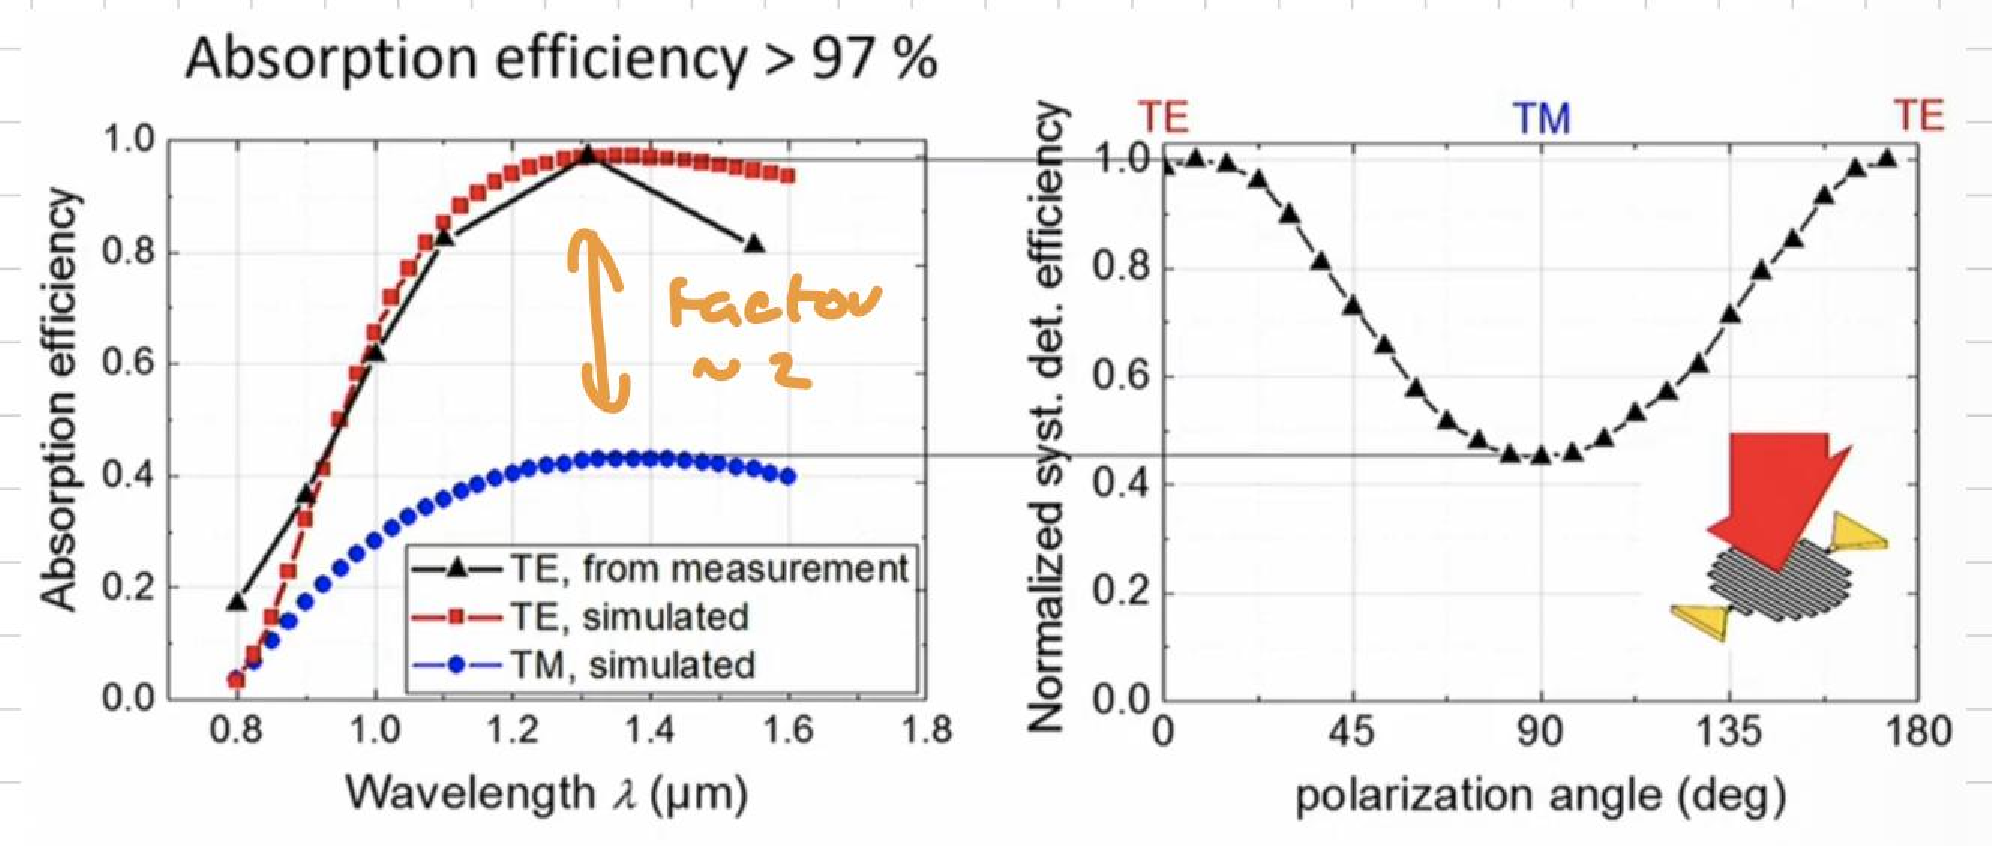
\includegraphics[width=0.8\linewidth]{images_in_pdf/8-/Grafico_47.pdf}
\end{figure}

The detector response can be different for \textbf{TE} (transverse electric) and \textbf{TM} (transverse magnetic) polarization, so the polarization must be taken into account carefully because it can strongly affect the absorption efficiency.
The time jitter depends on both electrical noise and geometry. Since the signal propagates through the detector with a finite speed, photons absorbed at different positions can produce pulses that arrive at slightly different times. The timing jitter is usually quantified by the full width at half maximum (FWHM) of the arrival-time distribution. For a Gaussian distribution, the FWHM is related to the standard deviation by
\[
\mathrm{FWHM} = 2\sqrt{2\ln 2}\,\sigma,
\]
and in optimized SNSPDs it can reach values of the order of a few picoseconds.